\documentclass{article}
\usepackage[utf8]{inputenc}
\usepackage{amsmath}
\usepackage{amssymb}
\usepackage{svg}
\usepackage{showlabels}

\usepackage{subfig}

\title{Bachelor}
\author{Lars Müller}
\date{February 2022}

\begin{document}

\maketitle

\section{Introduction}

A single layer perceptron is an affine function of the form 
\begin{equation}
    f: 	\mathbb{R}^n \xrightarrow{} \mathbb{R}^m
\end{equation}
\begin{equation*}
    f(x; W, b) = x W^T + b
\end{equation*}
where $x\in \mathbb{R}^{1 \times n} $, $W\in \mathbb{R}^{m \times n}$ and $ b \in \mathbb{R}^m$.
This is usually CITATION NEEDED followed by a nonlinear function $\phi$ because it allows us
to model nonlinearities in the data and approximate more complex functions.\\

In a Multilayer Perceptron $N$ single layer perceptrons are stacked and iteratively transform an input $x_0$.
Each layer $h_i, i \in \{1, ..., N\}$ is parametrized by the weight matrix $W_i$ and bias vector $b_i$ and computes
the input $x_{i+1}$ for the next layer. Layer $h_i$ is defined as:

\begin{equation}
    h_i: \mathbb{R}^n \xrightarrow{} \mathbb{R}^m
\end{equation}
\begin{equation*}\
    h_i(x_i; W_i, b_i) = \phi(f(x_i; W_i, b_i))
\end{equation*}
 
\noindent Multilayer perceptrons are a class of feed-forward neural networks.
\begin{figure}[htbp]
  \centering
  \includesvg[width = 150pt]{nn.svg}
  \caption{MLP Visualization for N = 3}
\end{figure}

\noindent The first layer is referred to as the input layer and the last one as the output layer. Layers between
these are called hidden layers.

\noindent The input and hidden layers choose from a variety of different nonlinear functions,
The most common one is a Rectified Linear Unit or ReLU for short due to their
favorable properties such as non-saturation of its gradient and its low compute cost.

\begin{equation}
    ReLU: \mathbb{R}^{n \times m} \xrightarrow{} \mathbb{R}^{n \times m}
\end{equation}
\begin{equation*}
    ReLU(x)=
        \begin{cases}
            0 &x\leq 0 \\
            x&\text{otherwise}
        \end{cases}
\end{equation*}

\noindent A common choice for the nonlinearity of the output layer is the $softmax$ function  to convert the 
logits that the MLP (Multilayer perceptron) computes to a probability distribution. 


\begin{equation}
    softmax: \mathbb{R}^K \xrightarrow{} \mathbb{R}^K
\end{equation}
\begin{equation*}
    softmax(x_N) = \frac{e^{y_j}}{\sum_{k=1}^K e^{y_k}}
\end{equation*}

where $K$ is the the dimension after the output layer.

\noindent A probability distribution as output of the neural network is commonly used in multiclass classification CITATION.
These can be used to determine how confident as neural network classifies a given input.
Low entropy of the distribution of $softmax(x_N)$ indicates a high confidence, while a high entropy
indicates a uniform distribution over the classes and therefore a low confidence.\\

\noindent One can also replace the single layer perceptron with a convolution layer if spatial invariance is helpful. The convolution network
has filters or kernel $a_i \in \mathbb{R}^{q \times r}$ which are applied from left to right, top to bottom
to the input $x$ and act as weight matrices. For notation purpose I will include the matrix indices in the exponent where $a_i^{j,k}$ refers
to the $j$'th row and the $k$'th column of $a_i$. This creates a result matrix $M_i$ for every filter $a_i$, whose rows and columns
will be indexed by $J$ and $K$ respectively.

\begin{equation}
    conv: \mathbb{R}^{n \times m} \xrightarrow{} \mathbb{R}^{o \times p}
\end{equation}
\begin{equation*}
    M_i^{J, K} = conv(x, J, K; a_i) = \sum_j^n \sum_k^m a_i^{j,k} x^{J - j, K - k}
\end{equation*}

\noindent This can be repeated for each layer, for multiple $a_i$ operating on multiple $M_j$, where $M$ is commonly
referred to as feature map. Convolution layers usually use ReLU as their nonlinearity
Due to their spatial invariance convolution layers see lots of popularity, especially on image data. CITATION
Perceptron layers and convolution layers can be combined in neural network architecture by reshaping the data.\newline

\noindent Neural networks are updated via Stochastic Gradient Descent on a loss function that defines the objective.
The gradient w.r.t. the parameters of the neural network is calculated and applied via an optimization algorithm such
as ADAM. This is done on subsets of the data, called minibatches.

\noindent Let $\phi_\theta: \mathbb{R}^{c \times n \times m} \xrightarrow{} \mathbb{R}^{k \times l}$ be a neural network consisting
of a combination of convolution and MLP layers which is parametrized by $\theta$. 

\begin{figure}[htbp]
  \centering
  \includesvg[width = 250pt]{convn.svg}
  \caption{Vizualization of an example $\phi$}
\end{figure}

\noindent To calculate the mean squared error loss $MSE$, 
we need input values  $x \in \mathbb{R}^{n\times m}$ and the true
label or the value you want to fit the network on $y \in \mathbb{R}^{n\times m}$.  
The output of our neural network $\phi_\theta(x)$ will be called $\hat{y}$. 
Mean squared error is mostly used in regression.

\begin{equation}
    MSE: \mathbb{R}^{n \times m} \xrightarrow{} \mathbb{R}
\end{equation}
\begin{equation*}
    MSE(y, \hat{y}) = \frac{1}{n} \sum_{i=0}^{n} (y_i-\hat{y}_i)^2
\end{equation*}

\noindent Another important loss is the cross-entropy loss $ce$. It is mainly used for multiclass classification and expects
probabilities over $k$ classes, so softmax is usually applied as the non-linearity of the output layer.
$y \in \{0, 1\}^{k}$ is a vector that contains the true class labels. $p \in [0, 1]^{k}$ contains
the per class probabilities that $\phi_\theta(x)$ predicts.
\begin{equation}
    ce: \mathbb{R}^{k} \xrightarrow{} \mathbb{R}
\end{equation}
\begin{equation*}
    ce(y, p) = \sum_{c=1}^My_{i}\log_2(p_{i})
\end{equation*}

\noindent If vanilla stochastic gradient descent is used as the optimization algorithm, the weights $\theta$
are updated via 
\begin{equation}
    \theta \xleftarrow{} \theta + \nabla \mathrm{loss}(y, \phi_\theta(x))
\end{equation}
\noindent In supervised learning $y$ is either obtainable by labeling data by hand or given
by some other source. If this is not an option different methods from
self-supervised and unsupervised learning can help create a target $y$.\newline
While unsupervised learning largely works without any target and is mostly used 
for clustering and dimensionality reduction, there are methods we can benefit from,
which will be discussed later.

\section{Self supervised learning}
For problems where data labeling is not feasible self-supervised learning or SSL
provides a way to obtain target and fit a $\phi$ on those. SSL also enables us
to pretrain neural networks and then switch to a downstream task by exposing the
supervised labels to it and fine tune $\phi$ on them. SSL autonomously creates
labels by using information from domain knowledge or correlations.\newline

\noindent SimCLR is a self supervised framework to form such targets for image data.
It allows us to learn a vector representation $r \in \mathbb{R}^{m}$ of the
input images $x \in \mathbb{R}^{n \times n}$ with $m \ll n^2$ .\newline
By applying a random transformation $t \sim T$ where $T$ is the set of all semantically 
invariant data augmentations to the image two views, denoted $\Tilde{x}_i$ and $\Tilde{x}_j$
are created.






Consider frames of the arcade game Ms. Pac-Man CITATION as the input data (Figure 3.)
\begin{figure}
    \centering
    \subfloat[Beginning of an Episode]{{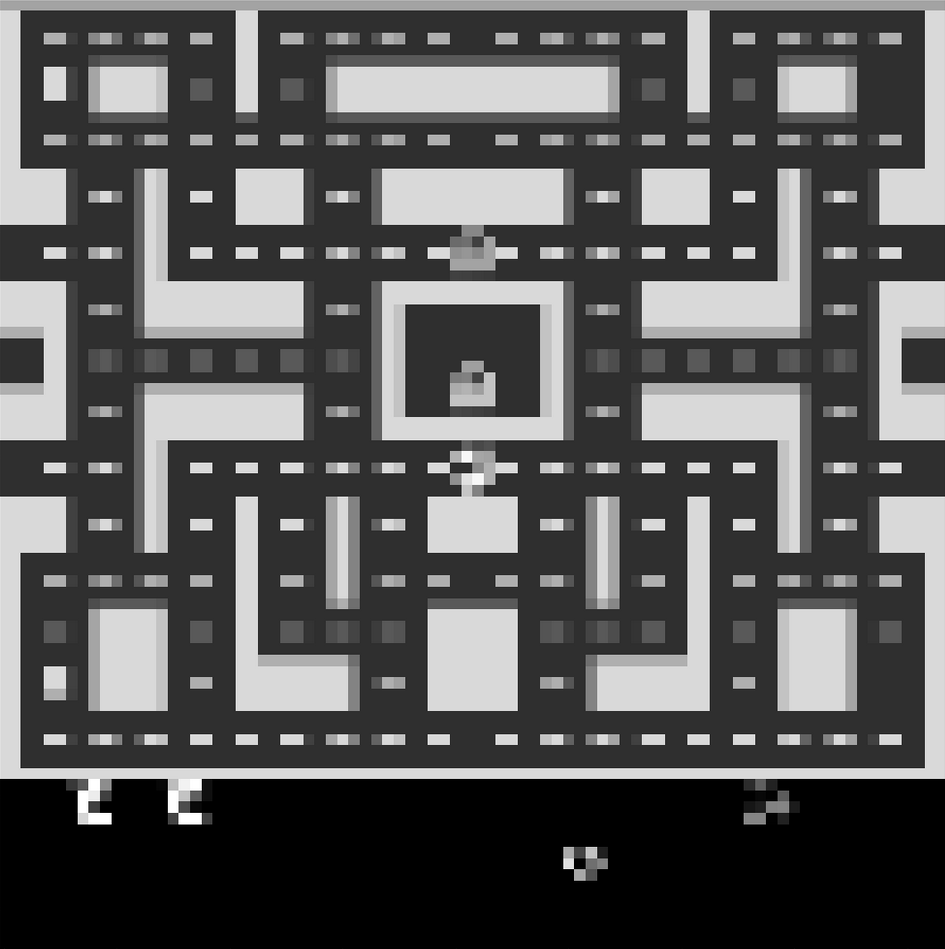
\includegraphics[width=5cm]{pacman_start.png} }}
    \qquad
    \subfloat[After 500 Frames have passed]{{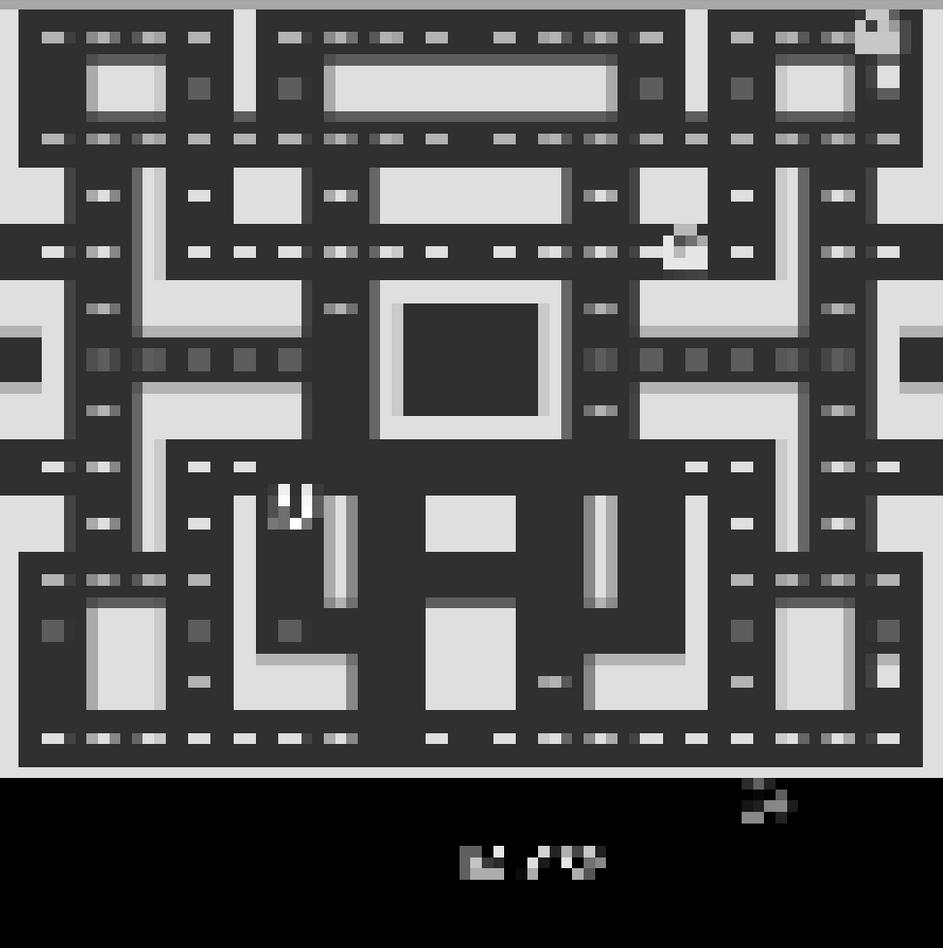
\includegraphics[width=5cm]{pacman.png} }}
    \caption{Frames from Ms. Pac-Man}
\end{figure}



Let $enc: \mathbb{R}^{n \times n} \xrightarrow{} \mathbb{R}^{m}$ be a neural network consisting of 
two convolution layers and a three layer MLP after the convolution. \newline




$$$$
\end{document}

